% Four-page ACM-format draft; references count toward the cap.
% Compile from this directory: tectonic main.tex
\documentclass[sigconf,nonacm]{acmart}
\usepackage{booktabs}
\emergencystretch=1.5em
\settopmatter{printacmref=false}
\setcopyright{none}
\renewcommand\footnotetextcopyrightpermission[1]{}
\pagestyle{plain}

\begin{document}
\title{Typed Decision Models as Passage Rerankers:\\Effectiveness, Calibration, and Context Selection}
\author{Parv Bhargava}
\affiliation{\institution{Independent Researcher}\country{}}
\email{parvbhargavapro@gmail.com}

\begin{abstract}
Typed decision models return probabilities over caller-defined options. We evaluate four families as pointwise passage rerankers on TREC DL 2019--2023 and eight BEIR collections, and study calibration and retrieval-augmented generation (RAG). Jev averages 56.1 nDCG@10 versus 56.0 for Qwen3-Reranker-8B and 53.7 for bge-reranker-v2-m3; pooled superiority and equivalence are sensitive to small-sample inference. Jev's raw yes/no probabilities reduce mean calibration error by five points on judged candidate pools, although source-label calibration gives bge a similar mean error. Same-base and context-budget controls constrain attribution to decision-model training. On 1,000 held-out questions each from MuSiQue and NQ with three generators, Jev improves multi-hop answer quality over bge, but probability thresholds do not improve on fixed top-$k$. These results support competitive ranking configurations, while showing that calibration alone does not ensure better context selection.
\end{abstract}
\keywords{reranking, decision models, calibration, retrieval-augmented generation}
\maketitle

\section{Introduction}
Rerankers score a small candidate pool after initial retrieval. Neural cross-encoders and label-probability language models are effective pointwise approaches; listwise systems instead order several passages together~\cite{sun2023rankgpt,qwen3embedding}. Typed decision models offer a related interface: the caller supplies a state and typed questions, and receives probabilities over defined options. Whether this interface delivers useful relevance probabilities, beyond competitive rankings, remains an empirical question.

We study Laya, Jeff, Clef, and Jev~\cite{laya,jeff,clef,jev} without task-specific tuning on our side. We ask: \textbf{RQ1}, how effective are they at reranking, including against same-base controls? \textbf{RQ2}, are their relevance probabilities calibrated, and can transfer calibration close the gap for conventional rerankers? \textbf{RQ3}, do these probabilities improve downstream context selection? Ranking, calibration, and answer quality require separate evaluation: a good ordering need not provide probabilities suitable for thresholding, and marginal passage relevance may miss multi-hop utility. We retain strong Qwen reranker baselines, controlled ablations, and uncertainty estimates to distinguish these claims.

\paragraph{Relation to prior work.}
Pointwise LLM ranking can use next-token probabilities over binary or graded labels~\cite{zhuang2023beyond}; our controls test whether a typed interface adds value beyond that readout. Earlier work studies Jev in recommendation reranking~\cite{lyu2026jevrec}, while evidence audits caution against attributing gains to the interface without comparable controls~\cite{tang2026tdmaudit}. Neural ranker scores can be poorly calibrated~\cite{penha2021calibration}. Rather than assess label agreement alone, we measure probability calibration and test its downstream utility against fixed-$k$ and score-gap selection~\cite{adaptivek2025}. We evaluate passage selection, not iterative retrieval or trained context compression.

\section{Methods and Evaluation}
\paragraph{Typed scores.}
Each query--passage pair is the model's state. Three questions request: Choice-3 (C3), with relevant, partially relevant, and irrelevant options; Noul, asking whether the passage answers or substantively addresses the query; and Score-4 (S4), with levels 0 (irrelevant), 1 (related), 2 (partly answering), and 3 (fully answering). Ranking scores are $(2p_{\rm rel}+p_{\rm part})/2$, $P(\mathrm{yes})$, and $\mathbb{E}[\ell]/3$, respectively. All three formats share one API call per pair, although Jeff evaluates them in separate forward passes; they are not independent samples. C3 adds $10^{-6}p_{\rm rel}$ as a secondary score; remaining exact ties use BM25 rank.

Calibration uses probabilities of binarized relevance, distinct from expected-grade ranking scores. Cross-encoder raw probabilities are sigmoid-transformed logits; calibration was not their training objective. Strict C3/S4 readouts are $p_{\rm rel}$/$P(\ell\ge2)$; lenient readouts add partial relevance/$P(\ell\ge1)$. The lenient policy for TREC-COVID, DBPedia, and News was introduced after observing poor strict C3 calibration. We therefore lead with policy-independent Noul and disclose both Jev C3 results (ECE 14.8 under the policy, 19.2 strictly).

\paragraph{Ranking suite and systems.}
We rerank identical Pyserini BM25 top-100 candidates from RankGPT/RankLLM~\cite{sun2023rankgpt,rankllm}: TREC DL19--23 (308 queries) and eight BEIR collections~\cite{thakur2021beir} (1,525 queries): TREC-COVID, NFCorpus, Touche, DBPedia, SciFact, Signal, News, and Robust04. The suite has 1,833 queries; 15 NFCorpus topics have empty BM25 candidate lists and score zero. Averages weight the 13 collections equally. Baselines include MiniLM-L6-v2 (22M), bge-reranker-v2-m3 (568M)~\cite{bgererankerv2m3}, and Qwen3-Reranker-0.6B/4B/8B~\cite{qwen3embedding} (4B/8B use 4-bit NF4). Decision models are Laya (421M), Jeff-Qwen3.5-0.8B v1.2, Clef 27B (seven collections), and closed Jev 1.13 (snapshot \texttt{20260917}). Additional controls use Qwen3-235B-A22B's yes/no and expected 0--4 token scores (eight collections), Clef's Qwen3.8-27B base (three), and Jeff's Qwen3.5-0.8B base (all 13), without decision interfaces~\cite{zhuang2023beyond}.

Cross-encoders use 512 total tokens; label-probability LLMs read 448 passage tokens. Jev/Clef/Jeff read 4,000 characters and Laya about 320 passage tokens. We additionally compare Jev and bge at 448 passage tokens on Touche, News, and Robust04, and extend bge to 2,048 tokens. Same-base comparisons thus assess configurations with differing prompts and contexts, rather than isolate training effects.

\paragraph{Metrics and inference.}
We report nDCG@10 and paired query-level $t$-tests, Holm-corrected across collections for each system--baseline pair. Random-effects pooling uses DerSimonian--Laird heterogeneity estimates, with normal and post-hoc modified Knapp--Hartung (mKH) intervals~\cite{rover2015mkh}; mKH uses $t_{k-1}$ and a residual variance multiplier floored at one. The $\pm2$ nDCG equivalence margin was chosen after observing results. Condensed nDCG excludes unjudged passages and cannot establish their relevance.

Calibration uses ECE (15 equal-width bins) and Brier score on judged pairs from nine collections containing negatives: DL19--23, TREC-COVID, DBPedia, News, Robust04. Relevant grades are $\ge2$ on DL and $\ge1$ on BEIR. Paired query-cluster bootstraps use 2,000 replicates and Holm over nine collections. Platt scaling~\cite{platt1999} fits $\sigma(a\,\mathrm{logit}(p)+b)$. Transfer uses source labels only: \emph{All} pools the other collections with equal pair weights; \emph{Group} balances source collections within the same numeric relevance-threshold group (DL or dense BEIR). Grouping does not imply identical relevance semantics. Target-label cross-fitted Platt scaling (10 repeated five-fold query splits) is a reference floor.

\begin{figure*}[t]
\centering
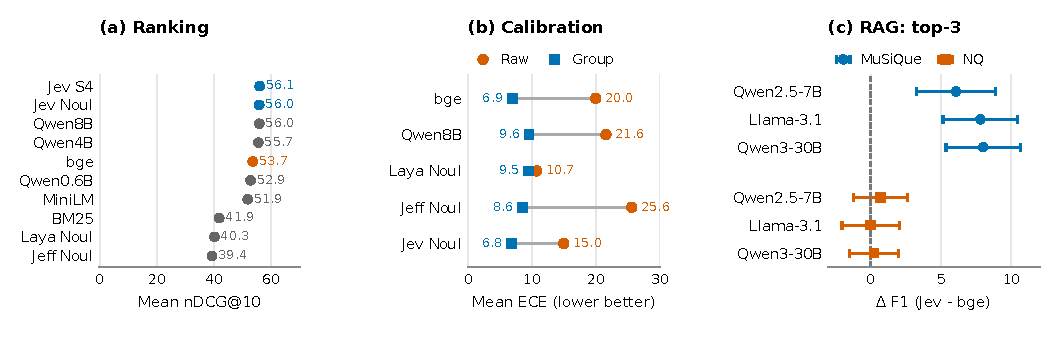
\includegraphics[width=\textwidth]{figures/results-overview.pdf}
\caption{Three views of the main results. (a) Equal-weight nDCG@10 means over 13 collections. (b) Raw versus numeric-group transfer ECE on nine judged candidate pools; decision-model readouts are Noul. Both metrics are in points. Means are descriptive. (c) Top-3 Jev--bge answer F1 differences on 1,000 questions per dataset, with ordinary paired 95\% CIs. All three MuSiQue effects pass Holm correction; none of the NQ top-3 effects do. Qwen denotes Qwen3-Reranker in (a,b).}
\label{fig:overview}
\end{figure*}

\begin{table*}[t]
\centering\footnotesize\setlength{\tabcolsep}{6pt}
\caption{Answer F1 on 1,000 held-out questions per dataset. Q2/L3/Q3 denote Qwen2.5-7B, Llama-3.1-8B, Qwen3-30B-A3B. $n$: mean passages selected. Every displayed paired Jev/bge policy favors Jev on MuSiQue (Holm $p<0.05$); on NQ, only L3 top-1 is significant. Thresholds are Platt-scaled using target calibration labels.}
\label{tab:rag}
\begin{tabular}{llrrrrrrrr}
\toprule &&\multicolumn{4}{c}{MuSiQue}&\multicolumn{4}{c}{NQ}\\
Ranker&Policy&Q2&L3&Q3&$n$&Q2&L3&Q3&$n$\\\midrule
--&All 20&38.8&37.0&46.3&20.0&52.5&49.4&51.5&20.0\\
--&Gold (oracle)&60.9&54.7&64.1&2.6&60.2&59.1&59.7&3.4\\
bge&Top-1&22.0&18.0&23.7&1.0&47.9&47.1&49.1&1.0\\
bge&Top-3&38.5&31.5&39.1&3.0&51.4&50.5&52.6&3.0\\
bge&Adaptive-$k$&30.5&26.1&32.6&3.1&50.6&50.5&51.8&7.1\\
bge&Top-2+$P>0.3$&35.7&30.4&37.9&2.9&51.3&51.2&52.6&3.9\\\addlinespace[2pt]
Jev&Top-1&45.2&36.4&43.4&1.0&50.4&50.4&51.4&1.0\\
Jev&Top-3&44.6&39.3&47.1&3.0&52.1&50.5&52.9&3.0\\
Jev&Adaptive-$k$&46.7&40.2&47.2&2.9&52.3&50.1&52.3&6.2\\
Jev&$P>0.3$&43.6&36.1&43.5&2.4&51.2&51.5&52.3&2.9\\
Jev&Top-2+$P>0.3$&44.2&39.1&45.2&3.0&51.8&51.0&53.2&3.5\\
\bottomrule
\end{tabular}
\end{table*}

\paragraph{RAG protocol.}
MuSiQue-Ans dev~\cite{trivedi2022musique} supplies 20 paragraphs with 2--4 supporting passages; NQ-open test~\cite{kwiatkowski2019nq} uses DPR top-20 passages~\cite{karpukhin2020dpr} and string-match answer labels; 18.6\% of final NQ questions have no answer-bearing candidate. Each dataset has seed-13 calibration/pilot/final splits of 200/300/1,000 questions. IDs are disjoint, but one related MuSiQue question with identical normalized wording crosses pilot/final under distinct IDs. Calibration labels choose Jev's readout by Brier score (Noul on MuSiQue, strict C3 on NQ) and fit Platt scaling. Even post-hoc \emph{raw} thresholds retain this label-selected readout.

Jev ranks by S4 and bge by its logit. Nine policies cover top-1/2/3/5, Adaptive-$k$ (largest score gap)~\cite{adaptivek2025}, $P>t$ with $t\in\{0.2,0.3\}$, and top-2 plus further passages with $P>t$, $t\in\{0.3,0.5\}$. Qwen2.5-7B-Instruct, Llama-3.1-8B-Instruct, and Qwen3-30B-A3B-Instruct-2507 generate short answers through OpenRouter (temperature 0; maximum 32 tokens; no abstention); we score SQuAD-normalized F1. Ranker-effect tests use paired questions, Holm over nine policies per dataset/generator. Threshold-rule tests use a separate four-comparison family. Policies were fixed after pilot; rule comparisons against top-3/Adaptive-$k$ were primary, while top-2/top-5 comparisons and raw thresholds were later exploratory additions. F1 equivalence tests with a post-hoc $\pm2$ margin are uncorrected. Full downstream comparisons cover bge, not Qwen8B.

\section{Results}

\paragraph{RQ1: Competitive but heterogeneous ranking.}
Jev S4's average is close to Qwen8B and above bge (Figure~\ref{fig:overview}a). On DL/BEIR, Jev averages 61.1/53.0 versus bge's 60.6/49.3. The pooled Jev--bge effect is $+2.6$ points: normal 95\% CI $[0.1,5.1]$, mKH $[-0.4,5.6]$. Jev--Qwen8B is $+0.3$: normal 90\% CI $[-1.3,1.9]$, mKH $[-1.4,2.02]$. Thus pooled superiority over bge and $\pm2$ equivalence to Qwen8B do not survive mKH. Heterogeneity is large ($I^2\approx0.9$). Collection-level Holm tests favor Jev over bge on five collections and none favor bge; against Qwen8B, Jev wins Robust04 ($+7.9$) but loses Signal ($-3.9$). BM25 remains best on Touche. Removing Robust04 reduces Jev/bge averages to 55.3/53.8; the mKH pooled 95\% CI still crosses zero ($[-0.4,3.9]$).

Clef and Jev average 64.4--65.4 and 64.1--65.2 across formats on seven shared collections; their exploratory equivalence survives mKH. Clef's base averages 75.5 on DL19/20 and TREC-COVID versus Clef's 74.8--75.5, with no significant collection-level difference, although mKH does not establish equivalence on only three collections. Jeff exceeds its base (39.1--39.4 vs.\ 31.8) but remains below BM25 overall. A graded readout improves Qwen235B from 58.1 to 59.8 on its eight collections, versus Jev S4 61.8. These are configuration comparisons.

At equal 448-token passage budgets, Jev exceeds bge on Robust04 ($+11.5$) and News ($+4.9$, both Holm $p<0.01$), and loses on Touche ($-9.9$). Extending bge largely closes the News gap but not Robust04. Separate newer-content checks yield Jev 62.5--63.5 versus bge 58.2 on FutureQueryEval~\cite{abdallah2025futurequery}, and 90.4--91.3 versus 81.8 on NovelEval~\cite{sun2023rankgpt}; leads over Qwen8B are not significant. Both sets predate Jev's release, so these checks cannot exclude contamination.

Published monoT5-3B results on identical candidates average 51.4 on BEIR-8 versus Jev S4's 53.0~\cite{nogueira2020monot5,sun2023rankgpt}. RankLLM reports a DL19--23 average of 62.1 for listwise RankZephyr-7B versus Jev's 61.1~\cite{rankllm,pradeep2023rankzephyr}. These comparisons are descriptive because matching published per-query outputs are unavailable; our 4-bit DL19 RankZephyr check scores 72.5 versus the published 74.1.

\paragraph{RQ2: Raw calibration gains can narrow after transfer.}
Jev Noul's mean raw ECE is 5.0 points below bge (bootstrap 95\% CI $[-6.3,-3.9]$), lower on eight of nine collections and significantly lower on five. Laya improves by 9.2 points; Jeff Noul is worse (Figure~\ref{fig:overview}b). Jev Noul also has lower mean Brier score (0.170 versus 0.215). Group transfer gives bge and Jev similar mean ECE (6.9/6.8), a descriptive comparison without a calibration-equivalence test. Pair-pooled transfer gives bge/Jev ECE 14.9/14.2. Jev and Laya's raw Noul advantage persists when unjudged candidates count as negatives, but calibration remains conditional on the candidate pool and labeling process. Their ECE advantages vary by less than 0.4 points across 5--30 bins and equal-mass binning. On seven shared collections, Clef C3 has raw ECE 7.8 and Brier 0.134 versus Jev C3 ECE 12.5 and bge 20.2; these subset means are separate from Figure~\ref{fig:overview}b.

\paragraph{RQ3: Ranking helps multi-hop RAG; thresholds do not.}
On MuSiQue, Jev beats bge by 2.6--23.2 F1 under all nine policies with all three generators (27 Holm-significant comparisons; Table~\ref{tab:rag} shows a subset and Figure~\ref{fig:overview}c plots top-3 gains). On NQ, only one of 27 differences is significant. Jev S4 puts the final supporting hop first on 51.2\% of MuSiQue questions versus bge's 15.2\%, despite a lower overall supporting-passage hit@1 (82.2\% vs.\ 88.0\%). This association helps characterize useful rankings but does not identify the cause. Gold-answer masking retains some final-hop preference, yet inserts an answer-location cue: 999/1,000 final-hop paragraphs carry the marker versus 1,621/19,988 candidates. It cannot isolate reasoning from memorization.

A pure Platt threshold $P>0.3$ leaves no context for 10.3\% of MuSiQue and 21.6\% of NQ questions. The top-2-plus-threshold rule selects 3.0/3.5 passages on average, saving none over top-3. It offers no significant gain over fixed top-$k$; post-hoc $\pm2$ F1 equivalence holds on NQ across generators, while MuSiQue results are equivalent to top-2 or slightly worse than larger/adaptive selections. Raw thresholds also fail to improve: on MuSiQue, raw $P>0.3$ leaves 25\% empty and is 3.4--5.9 F1 below top-3. Its readout still uses calibration labels. Jev's demonstrated downstream advantage over bge is chiefly ranking. The gap to gold-context answers remains substantial, so choosing a useful single passage does not solve multi-hop evidence selection.

\section{Discussion and Conclusion}
Typed decision models can be competitive passage rerankers, but neither their interface nor lower raw ECE guarantees improved context selection. Strong trained rerankers remain essential comparisons; the full RAG study establishes no advantage over Qwen8B. Same-base controls do not isolate decision training, and long-document gains vary by collection.

\paragraph{Efficiency.}
Local models ran on an 8\,GB RTX 4060. Median pair-scoring latency ranges from 0.3--14\,ms for the small trained rerankers to 102/148\,ms for 4-bit Qwen4B/8B. Jev takes 176\,ms per API call with concurrent requests; hardware and serving differ, so these are indicative rather than controlled speed comparisons. Jev averages \$3.4 per 1,000 queries at depth 100; all API experiments cost about \$31. Smaller generator contexts exclude candidate-scoring costs.

\paragraph{Limits and reproducibility.}
We use BM25 candidates, one prompt per format, and no task-specific tuning. Incomplete qrels, propagated DL22 judgments, and 31 synthetic DL23 queries constrain interpretation. Jev's size, training data, and cutoff are unknown; collection contamination remains possible. Generator providers may differ in quantization, and historical weight revisions were not recorded. We retain cached runs, complete input hashes, split IDs, and analysis scripts for numerical verification. The disclosed pilot/final overlap and post-hoc analyses constrain inference. Future work should use semantically grouped splits, matched contexts, and a strong downstream Qwen8B baseline.

\clearpage
\bibliographystyle{ACM-Reference-Format}
\bibliography{refs}
\end{document}
